\section{Aufbau}
\label{sec:Aufbau}
Benötigt werden ein Laser, in diesem speziellen Fall ein He-Ne-Laser, der mit Hilfe eines Polarisationsfilters polarisiert wird, ein Spiegel auf einem Goniometer, ein schwenkbares Photoelement, welches an einem Amperemeter angeschlossen wird. 
\begin{figure}
    \centering
    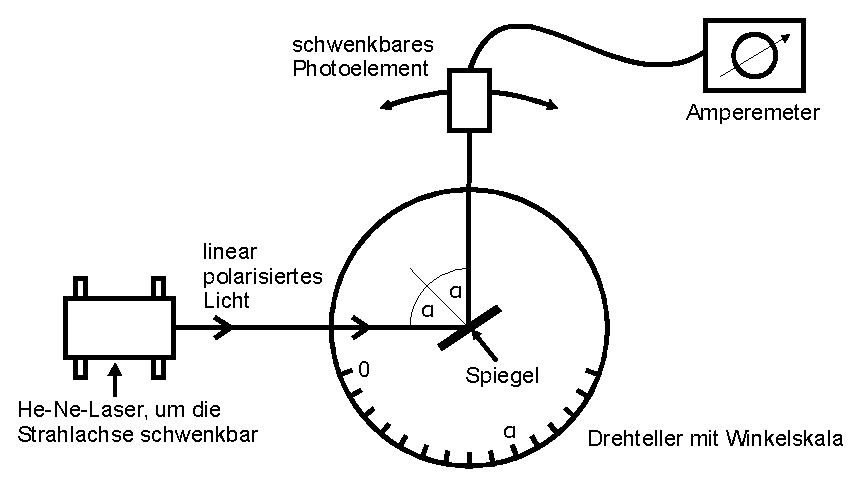
\includegraphics[height = 6cm]{GesamtAufbau.pdf}
    \caption{Aufbau der Messapparatur}
    \labe{fig:GesamtAufbau}
\end{figure}
Der Aufbau ist in \autoref{fig:GesamtAufbau}schematisch dargestellt.

In \autoref{fig:AufbauKlein} ist die Drehplatte dargestellt.
\begin{figure}
    \centering
    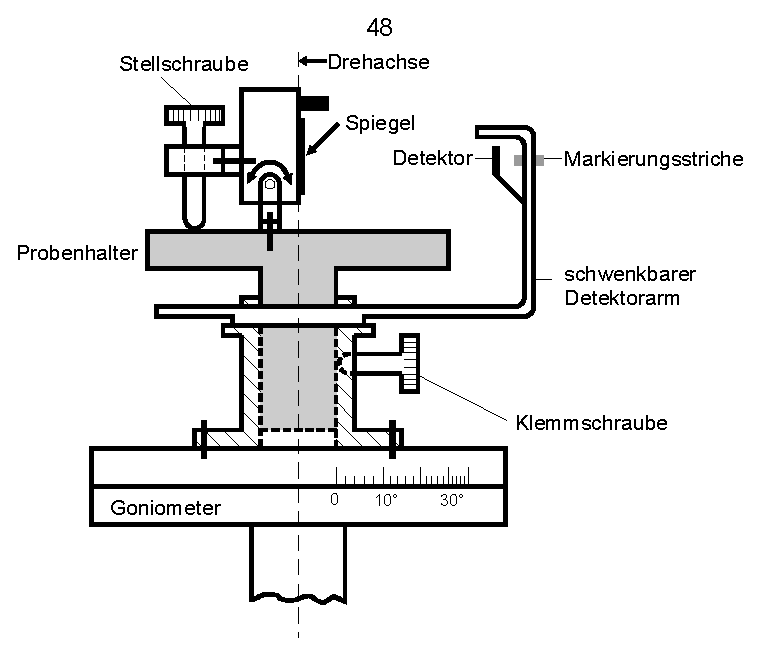
\includegraphics[height = 6cm]{AufbauKlein.pdf}
    \caption{Aufbau der Drehplattform}
    \label{fig:AufbauKlein}
\end{figure}
Auf dem Goniometer wird die Probenhalterung befestigt. AUf dieser wird der Spiegel mit einer Stellschraube befestigt. Unterhalb dieses Probenhalters wird der schwenkbare Detektorarm befestigt.
